\documentclass[oneside,14pt]{extarticle}
\usepackage{cmap}
\usepackage[utf8]{inputenc}
\usepackage[english,ukrainian]{babel}
\usepackage{graphicx}
\usepackage{geometry}
\usepackage{listings}
\usepackage{float}
\usepackage{amsmath}
\usepackage{subfig}
\geometry{
	a4paper,
	left=20mm,
	right=20mm,
	top=15mm,
	bottom=15mm,
}
\lstset{
	language=c,
	tabsize=4,
	keepspaces,
	showstringspaces=false,
	frame=single,
	language=C,
}
\graphicspath{ {./pictures} }
\setlength{\parindent}{4em}

\newcommand\subject{Основи програмування вбудованих систем}
\newcommand\lecturer{доцент кафедри ПЗ\\Марусенкова Т.А.}
\newcommand\teacher{доцент кафедри ПЗ\\Крук О.Г.}
\newcommand\mygroup{ПЗ-32}
\newcommand\lab{1}
\newcommand\theme{Дослідження середовища Keil і бібліотек CMSIS і SPL (на прикладі блимання світлодіодами).}
\newcommand\purpose{Ознайомитися з можливостями середовища Keil uVision}

\begin{document}
\begin{normalsize}
	\begin{titlepage}
		\thispagestyle{empty}
		\begin{center}
			\textbf{МІНІСТЕРСТВО ОСВІТИ І НАУКИ УКРАЇНИ\\
				НАЦІОНАЛЬНИЙ УНІВЕРСИТЕТ "ЛЬВІВСЬКА ПОЛІТЕХНІКА"}
		\end{center}
		\begin{flushright}
			\textbf{ІКНІ}\\
			Кафедра \textbf{ПЗ}
		\end{flushright}
		\vspace{80pt}
		\begin{center}
			\textbf{ЗВІТ}\\
			\vspace{10pt}
			до лабораторної роботи № \lab\\
			\textbf{на тему}: <<\textit{\theme}>>\\
			\textbf{з дисципліни}: <<\subject>>
		\end{center}
		\vspace{80pt}
		\begin{flushright}
			
			\textbf{Лектор}:\\
			\lecturer\\
			\vspace{28pt}
			\textbf{Виконав}:\\
			
			студент групи \mygroup\\
			Коваленко Д.М.\\
			\vspace{28pt}
			\textbf{Прийняв}:\\
			
			\teacher\\
			
			\vspace{28pt}
			«\rule{1cm}{0.15mm}» \rule{1.5cm}{0.15mm} 2024 р.\\
			$\sum$ = \rule{1cm}{0.15mm}……………\\
			
		\end{flushright}
		\vspace{\fill}
		\begin{center}
			\textbf{Львів — 2024}
		\end{center}
	\end{titlepage}
		
	\begin{description}
		\item[Тема.] \theme.
		\item[Мета.] \purpose.
	\end{description}

	\section*{Індивідуальне завдання}
	6. Почергове циклічне увімкнення жовтого, зеленого, синього та червоного світлодіодів.

	\section*{Теоретичні відомості}
	6. Як відстежити значення змінної у середовищі Keil?
	
	В режимі \textit{Debug} відкрити вікно \textit{View->Watch->Watch 1} та у полі \textit{Enter expression} ввести назву змінної.
	
	\section*{Хід роботи}
	\subsection*{Створення проекту}
	\begin{figure}[H]
		\centering
		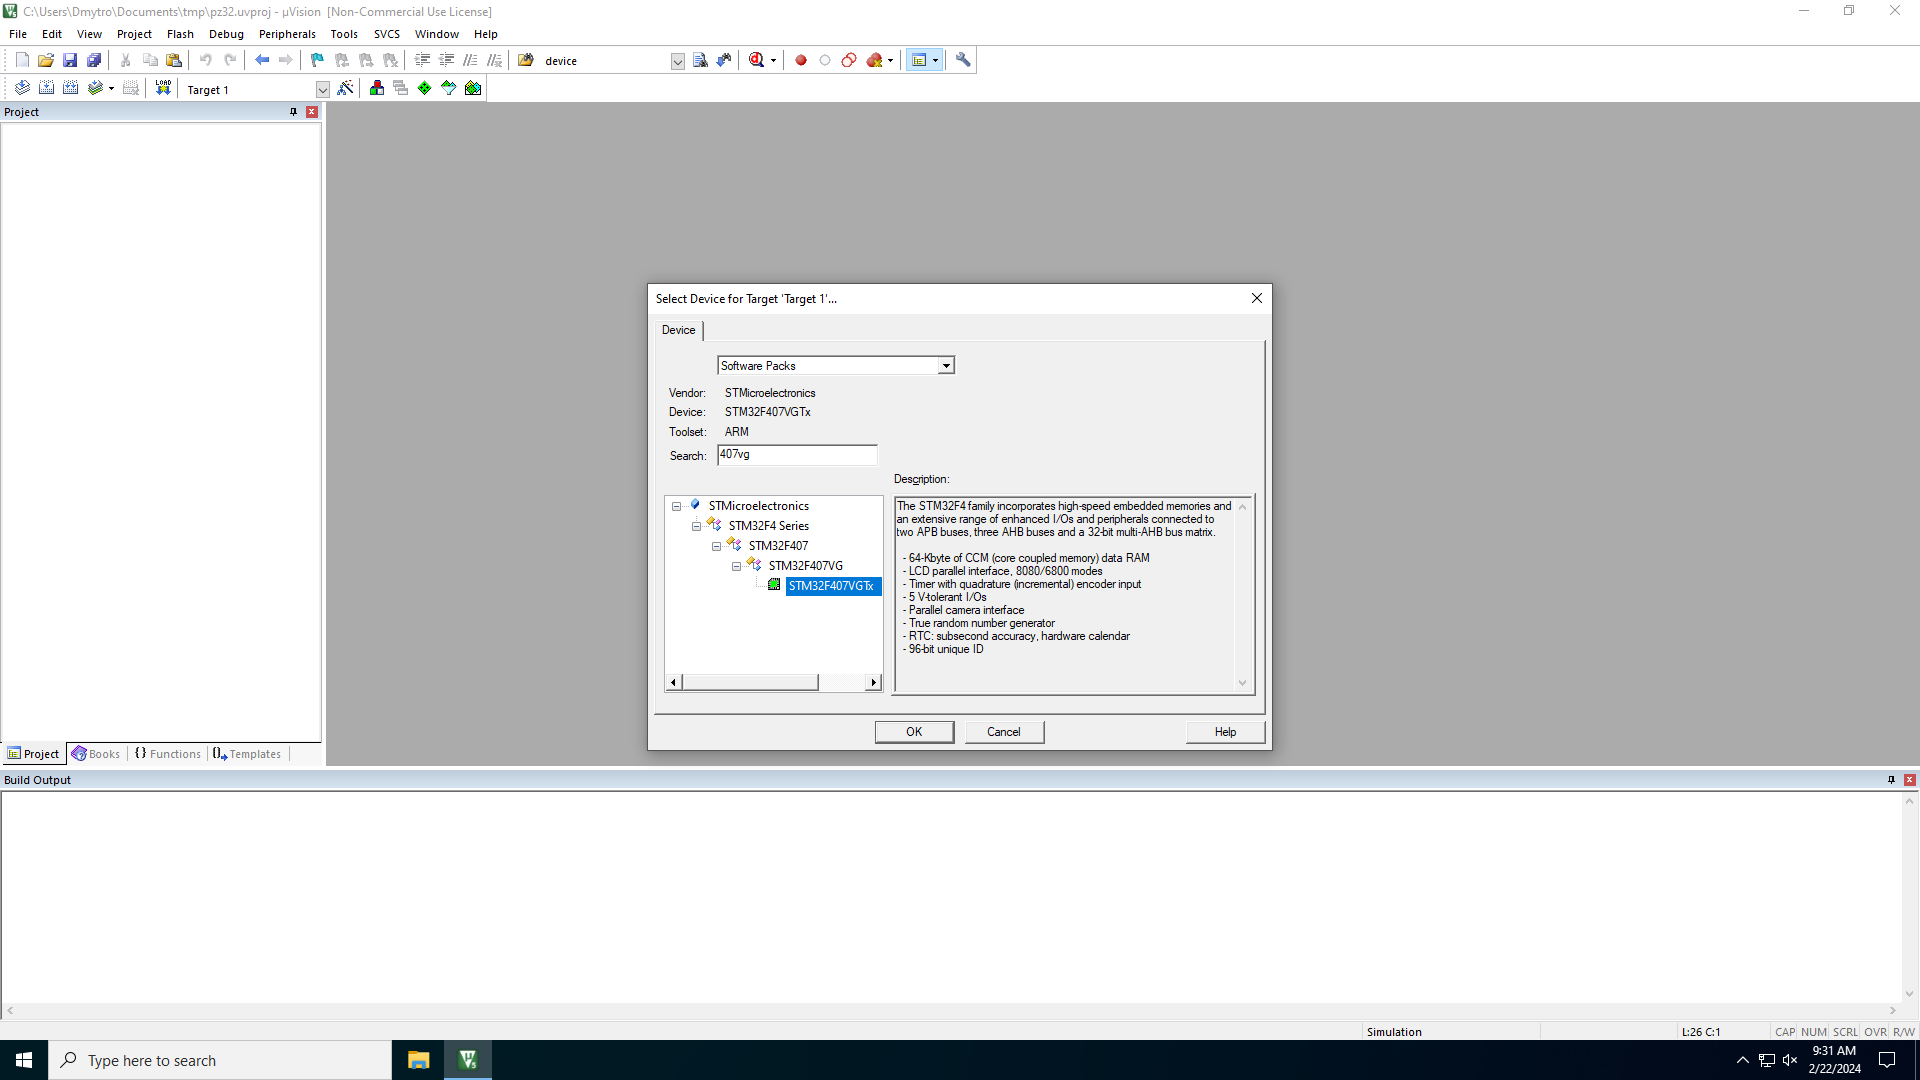
\includegraphics[scale=0.3]{1}
		\caption{Вибір девайсу після встановлення розширення STM.}
	\end{figure}
	
	\begin{figure}[H]
		\centering
		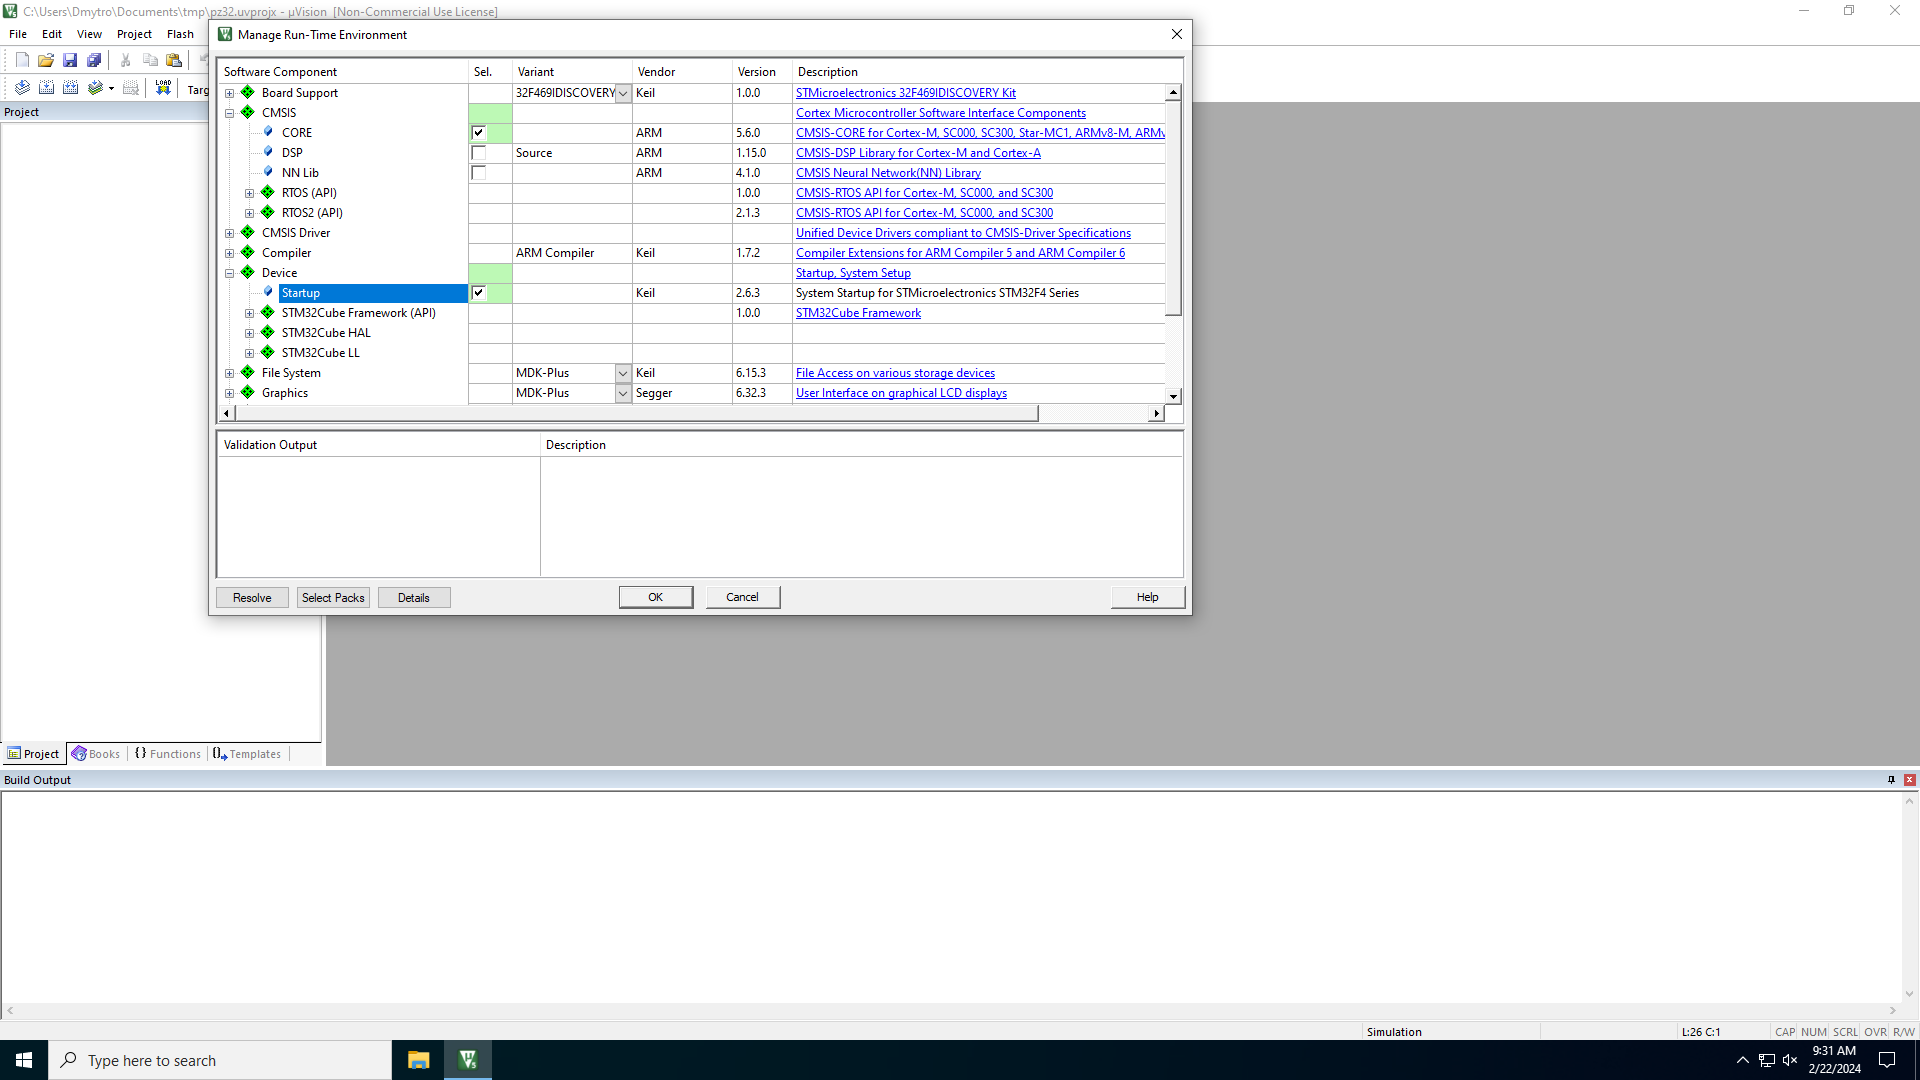
\includegraphics[scale=0.3]{2}
		\caption{Вибір компонентів для проекту.}
	\end{figure}
	
	\begin{figure}[H]
		\centering
		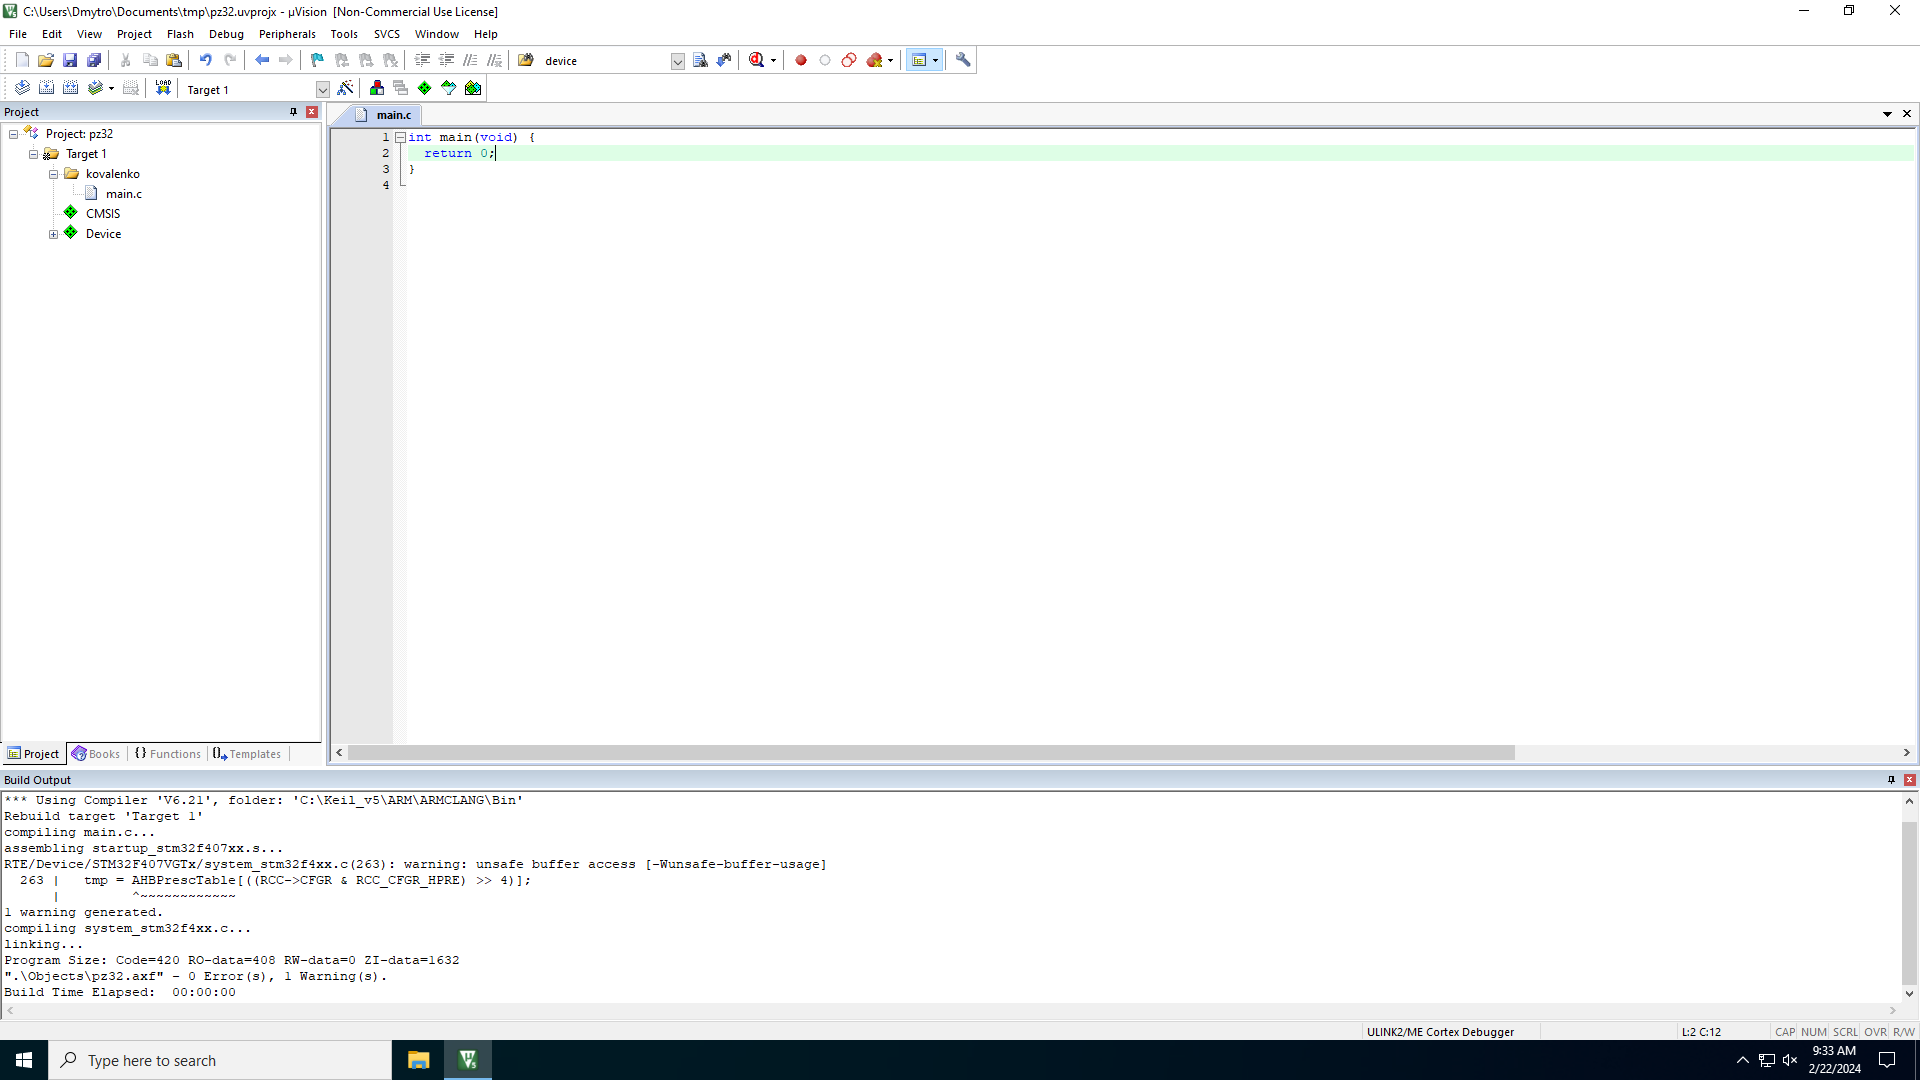
\includegraphics[scale=0.3]{3}
		\caption{Новий проект, що нічого не виконує.}
	\end{figure}
	
	\begin{figure}[H]
		\centering
		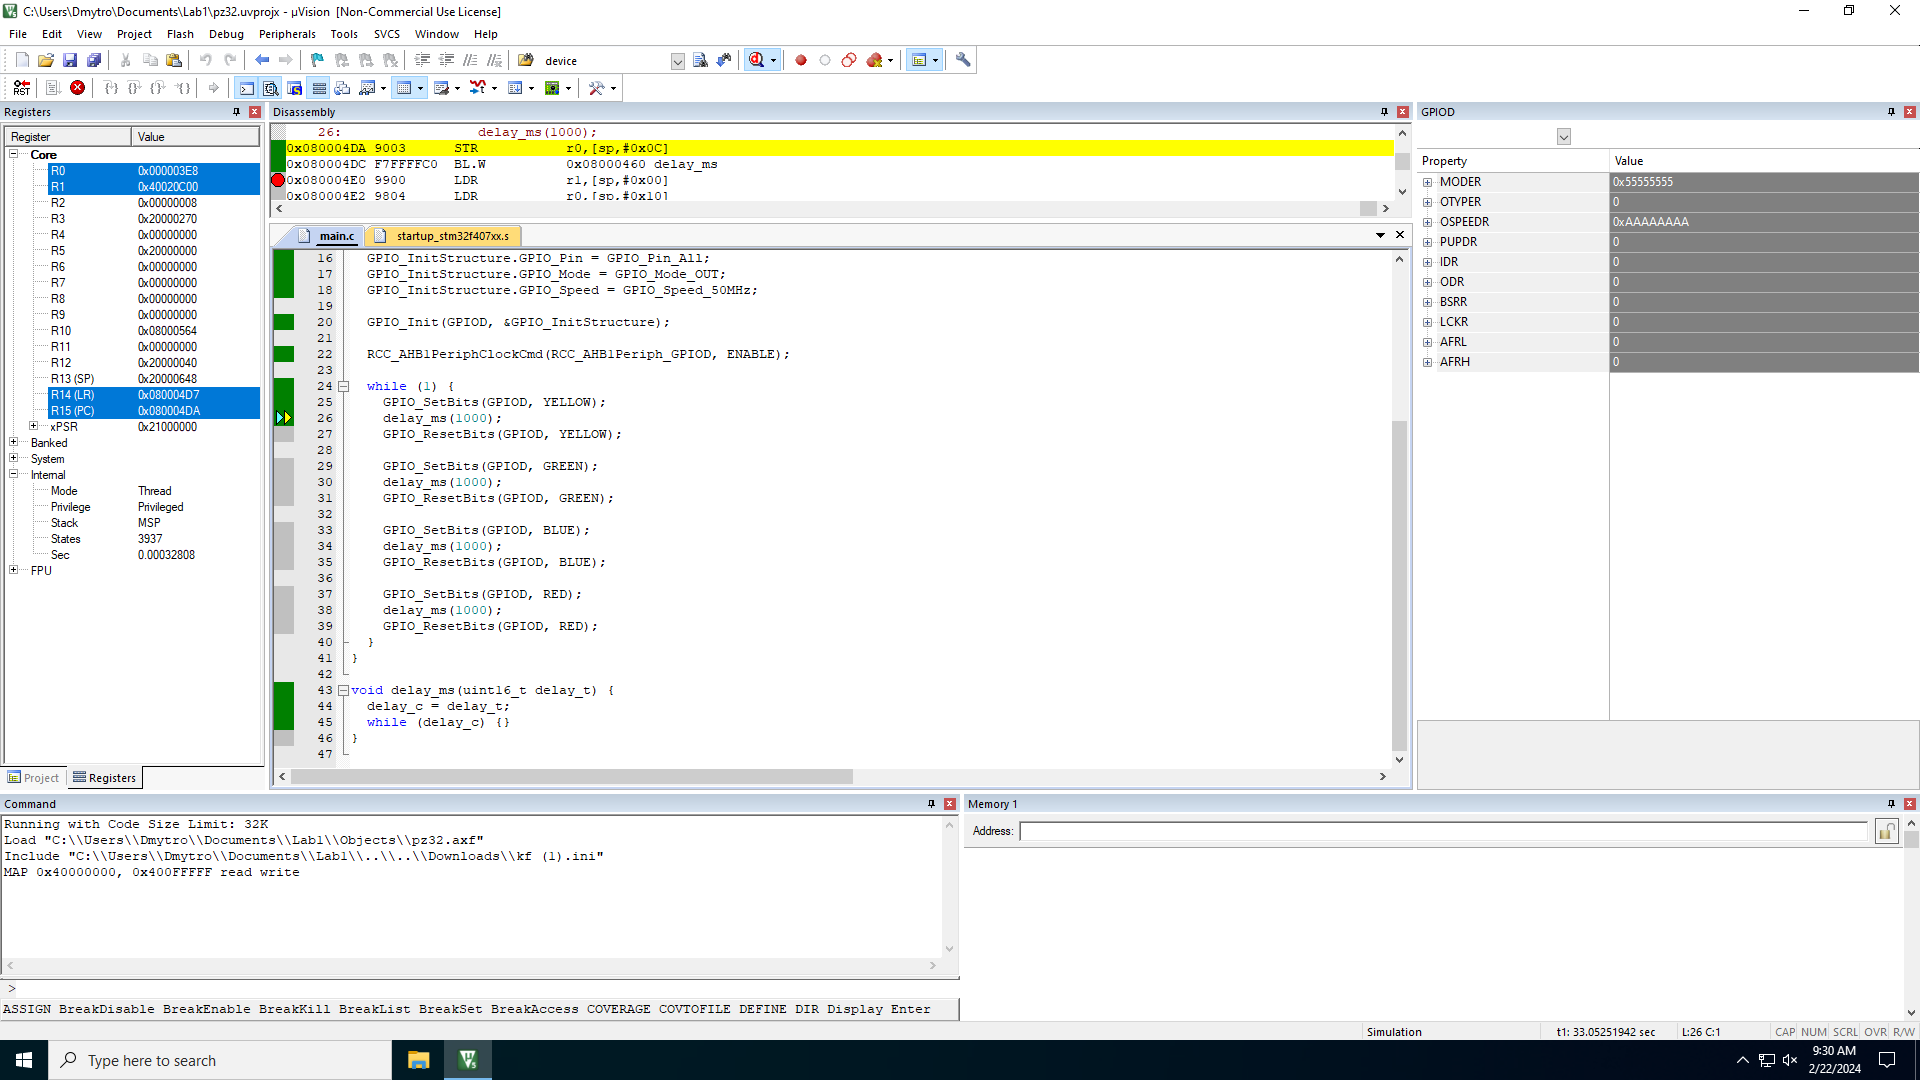
\includegraphics[scale=0.3]{4}
		\caption{Виконання коду програми в режимі Debug.}
	\end{figure}

	\subsection*{Код програми}
	Файл \textit{main.c}:
	{\small
		\begin{lstlisting}
#include "stm32f4xx.h"
#include "stm32f4xx_rcc.h"
#include "stm32f4xx_gpio.h"

#define YELLOW GPIO_Pin_12
#define GREEN GPIO_Pin_13
#define BLUE GPIO_Pin_14
#define RED GPIO_Pin_15

void delay_ms(uint16_t delay_t);

static GPIO_InitTypeDef GPIO_InitStructure;
static uint16_t delay_c = 0;

int main (void){
	GPIO_InitStructure.GPIO_Pin = GPIO_Pin_All;
	GPIO_InitStructure.GPIO_Mode = GPIO_Mode_OUT;
	GPIO_InitStructure.GPIO_Speed = GPIO_Speed_50MHz;
	
	GPIO_Init(GPIOD, &GPIO_InitStructure);
	
	RCC_AHB1PeriphClockCmd(RCC_AHB1Periph_GPIOD, ENABLE);
	
	while (1) {
		GPIO_SetBits(GPIOD, YELLOW);
		delay_ms(1000);
		GPIO_ResetBits(GPIOD, YELLOW);
		
		GPIO_SetBits(GPIOD, GREEN);
		delay_ms(1000);
		GPIO_ResetBits(GPIOD, GREEN);
		
		GPIO_SetBits(GPIOD, BLUE);
		delay_ms(1000);
		GPIO_ResetBits(GPIOD, BLUE);
		
		GPIO_SetBits(GPIOD, RED);
		delay_ms(1000);
		GPIO_ResetBits(GPIOD, RED);
	}
}

void delay_ms(uint16_t delay_t) {
	delay_c = delay_t;
	while (delay_c) {}
}
		\end{lstlisting}
	}
	
	\section*{Висновки}
	Під час виконання лабораторної роботи я ознайомився з можливостями середовища Keil uVision та дослідив середовище Keil і бібліотеи CMSIS і SPL створивши програму для почергового блимання жовтим, зеленим, синім та червоним світлодіодами.
	    
\end{normalsize}
\end{document}
